\chapter{Toward a new millennium}
\label{ch.otlabphon}

The period covered in chapters~\ref{ch.genphon} and~\ref{ch.spe}
above, from the 1950s through the early 1970s, saw not only a
significant re-orientation of direction in linguistics, and phonology
in particular, but also major growth in the overall field. Membership
in the {Linguistic Society of America},\footnote{The numbers cited here
  cover the field only in the United States, on the basis of data
  available in the Annual Reports of the LSA and its Directories of
  University Resources and Programs, the primary sources available to
  me. Note that LSA membership figures include many scholars in
  language departments, ESL programs, and other areas not
  representative of core theoretical study. Note also that the number
  of programs cited below almost certainly represents an undercount,
  since the volumes from which they are derived report that many
  institutions failed to submit information in response to requests.}
starting at 301 after its first year of existence, more than doubled
from 839 in 1951 to 1768 in 1960, and grew to 4723 in 1971, remaining
over 4000 through the 1970s and 1980s, reaching a peak of 4788 in
1990. Attendance at the LSA's Annual Meeting grew from a convivial 65
in 1950 to 198 in 1960 and exploded to 921 in 1969; from then on the
numbers are heavily dependent on the venue chosen for the meeting, but
generally range between 400 and the all time high of 1200 for the 1981
meeting in New York.
\begin{figure}[h]
  \centering
  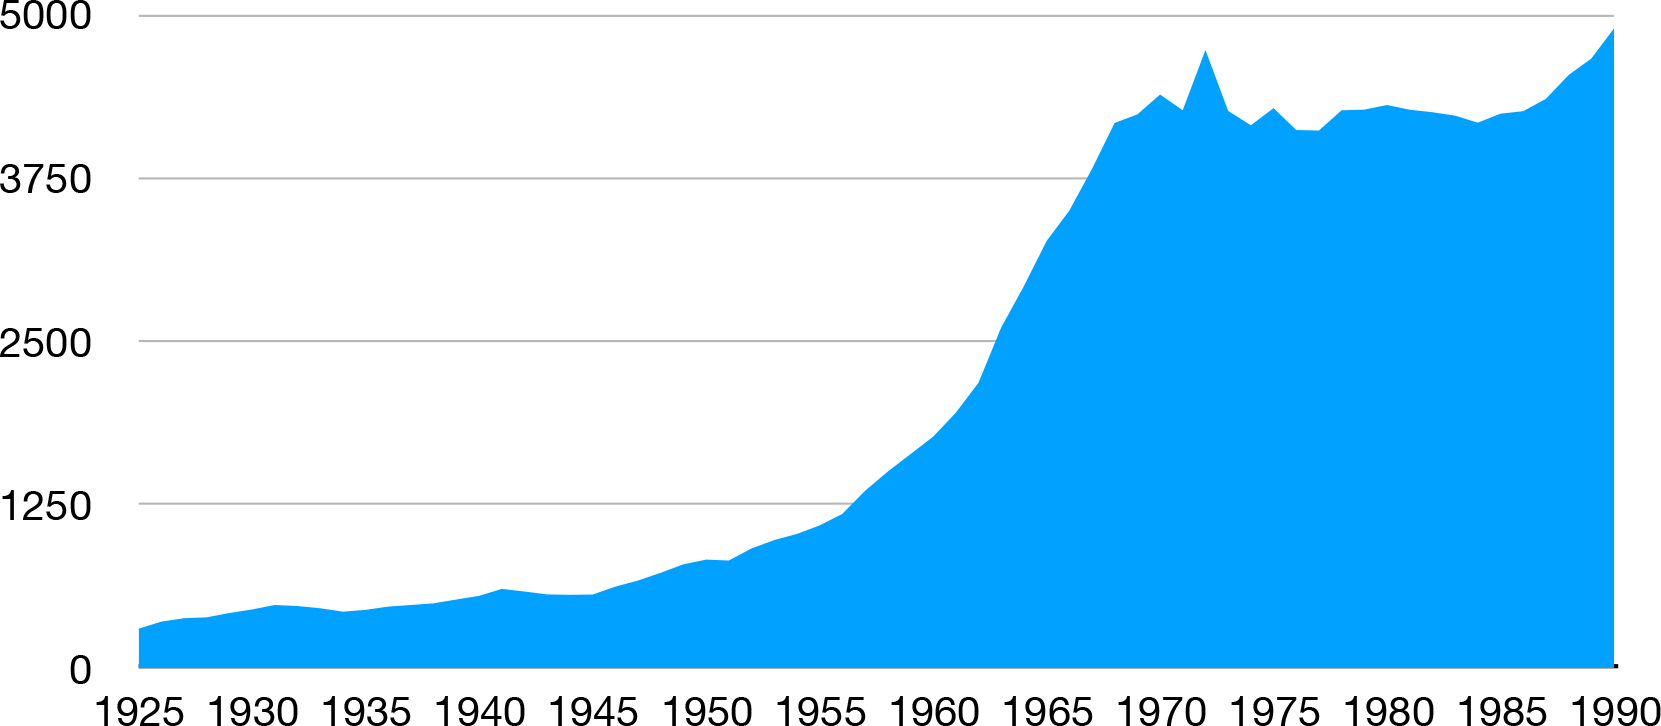
\includegraphics[width=.8\textwidth]{figures/LSA1925-90.jpg}
  \caption{LSA Membership 1925--1990}
  \label{fig:lsa.membership}
\end{figure}

The number of programs offering degrees in linguistics also grew
steadily. In 1962 these included 6 for the BA/BS, 22 for the MA/MS and
19 for the PhD; by 1969 there were 112 institutions offering the
BA/BS, 64 MA/MS, 45 PhD; in 1978: 115 BA/BS, 83 MA/MS, 49 PhD; and in
1982 135 BA/BS, 109 MA/MS, 73 PhD.  From this it follows that the
number of students pursuing research in linguistics also grew
considerably. A somewhat imperfect index of this is provided by
information about the number of student members of the LSA, which grew
from 52 in 1953 (the earliest available data year) to 299 in 1963 and
a peak of 1070 in 1973, remaining between 800 and 1000 through the
1970s and 1980s.

This overall growth in the number of research scholars naturally
resulted in a growing hunger for research topics that they could
pursue, and a theme of the present chapter will be that the flowering
of large numbers of distinct theoretical issues and positions seen in
the post-\textsl{\isi{SPE}} decades of the twentieth century is closely
connected with this matter of scholarly demographics.

Within a few years after the publication of \textsl{\isi{SPE}} and the
responses to its program discussed in chapter~\ref{ch.spe}, there was
broad enough discontent among phonologists to encourage students to
look elsewhere. The problem of how to represent the \isi{naturalness} of
rules and segment inventories, for example, largely disappeared from
the literature, along with the notational issues that seemed so
prominent in the late 1960s and early 1970s. Even the issue of
\isi{abstractness} ceased to be a focus of discussion. None of these areas,
it should be stressed, lost the attention of phonologists because of a
feeling that their problems had essentially been solved: on the
contrary, after a little reflection, most linguists would agree that
there remain significant unresolved questions in a number of areas
that held center stage earlier. Rather, what happened seems to have
been that attention was simply diverted by the exciting possibilities
inherent in the major innovations of subsequent years.

On the one hand, the \textsl{\isi{SPE}} program itself offered few obvious
topics for significant advances. The challenges posed by matters of
\isi{notational conventions} and rule ordering were highly technical, and
difficult to address in terms of readily accessible empirical evidence
--- difficulties similar to those presented by \isi{phonemic theory} a
decade or so earlier. On the other hand, the attempts to deal with
limitations of the \textsl{\isi{SPE}} program within its general
\emph{Weltanschauung} all seemed unappealing for reasons of their
own. The climate was ripe for a more serious re-orientation of
theoretical attention.

\section{A focus on representations}
\label{sec:representations}

This found its expression in the re-orientation of phonological
research over the next two decades from the study of phonological rule
systems to the study of \isi{representations}. \textsl{\isi{SPE}} and related
theories were built on the assumption that phonological (and phonetic)
\isi{representations} took the form of sequences of segmental units, each
composed of values for features taken from a universally available
set. The result could be represented as a matrix whose rows correspond
to the features and whose columns to the successive segments. The only
units larger than the segment that were recognized on this view were
morphological in character (morphemes, words, etc.); and they were
represented not directly as structural units but, rather, by the
intercalation of segmentoid \isi{boundaries} in the segmental string so as
to delimit one such unit from its neighbors. No structure internal to
the segment was recognized (aside from the fact that segments
themselves were regarded as internally unordered collections of
features), and no structural units larger than segments (such as
syllables) had any systematic representational status.

A variety of challenges arose to this formally simple mode of
representation, each presenting the possibility of new research
problems for investigation and new solutions to old problems. In each
case the novel vista provided a certain amount of low hanging fruit
for exploitation by a generation of graduate students and others; once
that had been gathered, the tendency was to look for other novelties,
and the field was quite prepared to provide these.

\subsection{Metrical Phonology and structure above the segment}
\label{sec:smetrical-phon}


One of the earliest successes of (what would become) the generative
approach to phonology was the elegant analysis of \ili{English} \isi{stress}
provided by \citet{chomsky:halle:lukoff}, an account which evolved
into that of \citet{spe}. The apparatus necessary to support this
picture, however, presented some problems. Since features in the
\textsl{\isi{SPE}} framework were associated with individual columns
(segments) in the representation, this resulted in \isi{stress} values being
associated only with a single vowel, rather than with an entire
\isi{syllable} --- and indeed, syllables had no status at all in this
theory. Furthermore, the feature {[Stress]}, unlike others, was
required to take a range of numeric values, rather than a binary
choice between `$+$' and `$-$'; and a rather unwieldy convention of
\isi{stress} reduction had to be posited such that assignment of {[1Stress]}
anywhere within a form resulted in the demotion of all other values
from {[\emph{n}Stress]} to {[\emph{n}+1Stress]}.

A solution to these difficulties was provided by Mark
\posscitet{liberman75:thesis} MIT dissertation, the results of which
were included in \posscitet{liberman:prince:stress} foundational
published presentation. There it was proposed that instead of a single
homogeneous matrix of features, a phonological representation should
be regarded as a binary branching tree whose terminal elements were
prosodic constituents: syllables.

\begin{wrapfigure}{l}{.35\textwidth}
  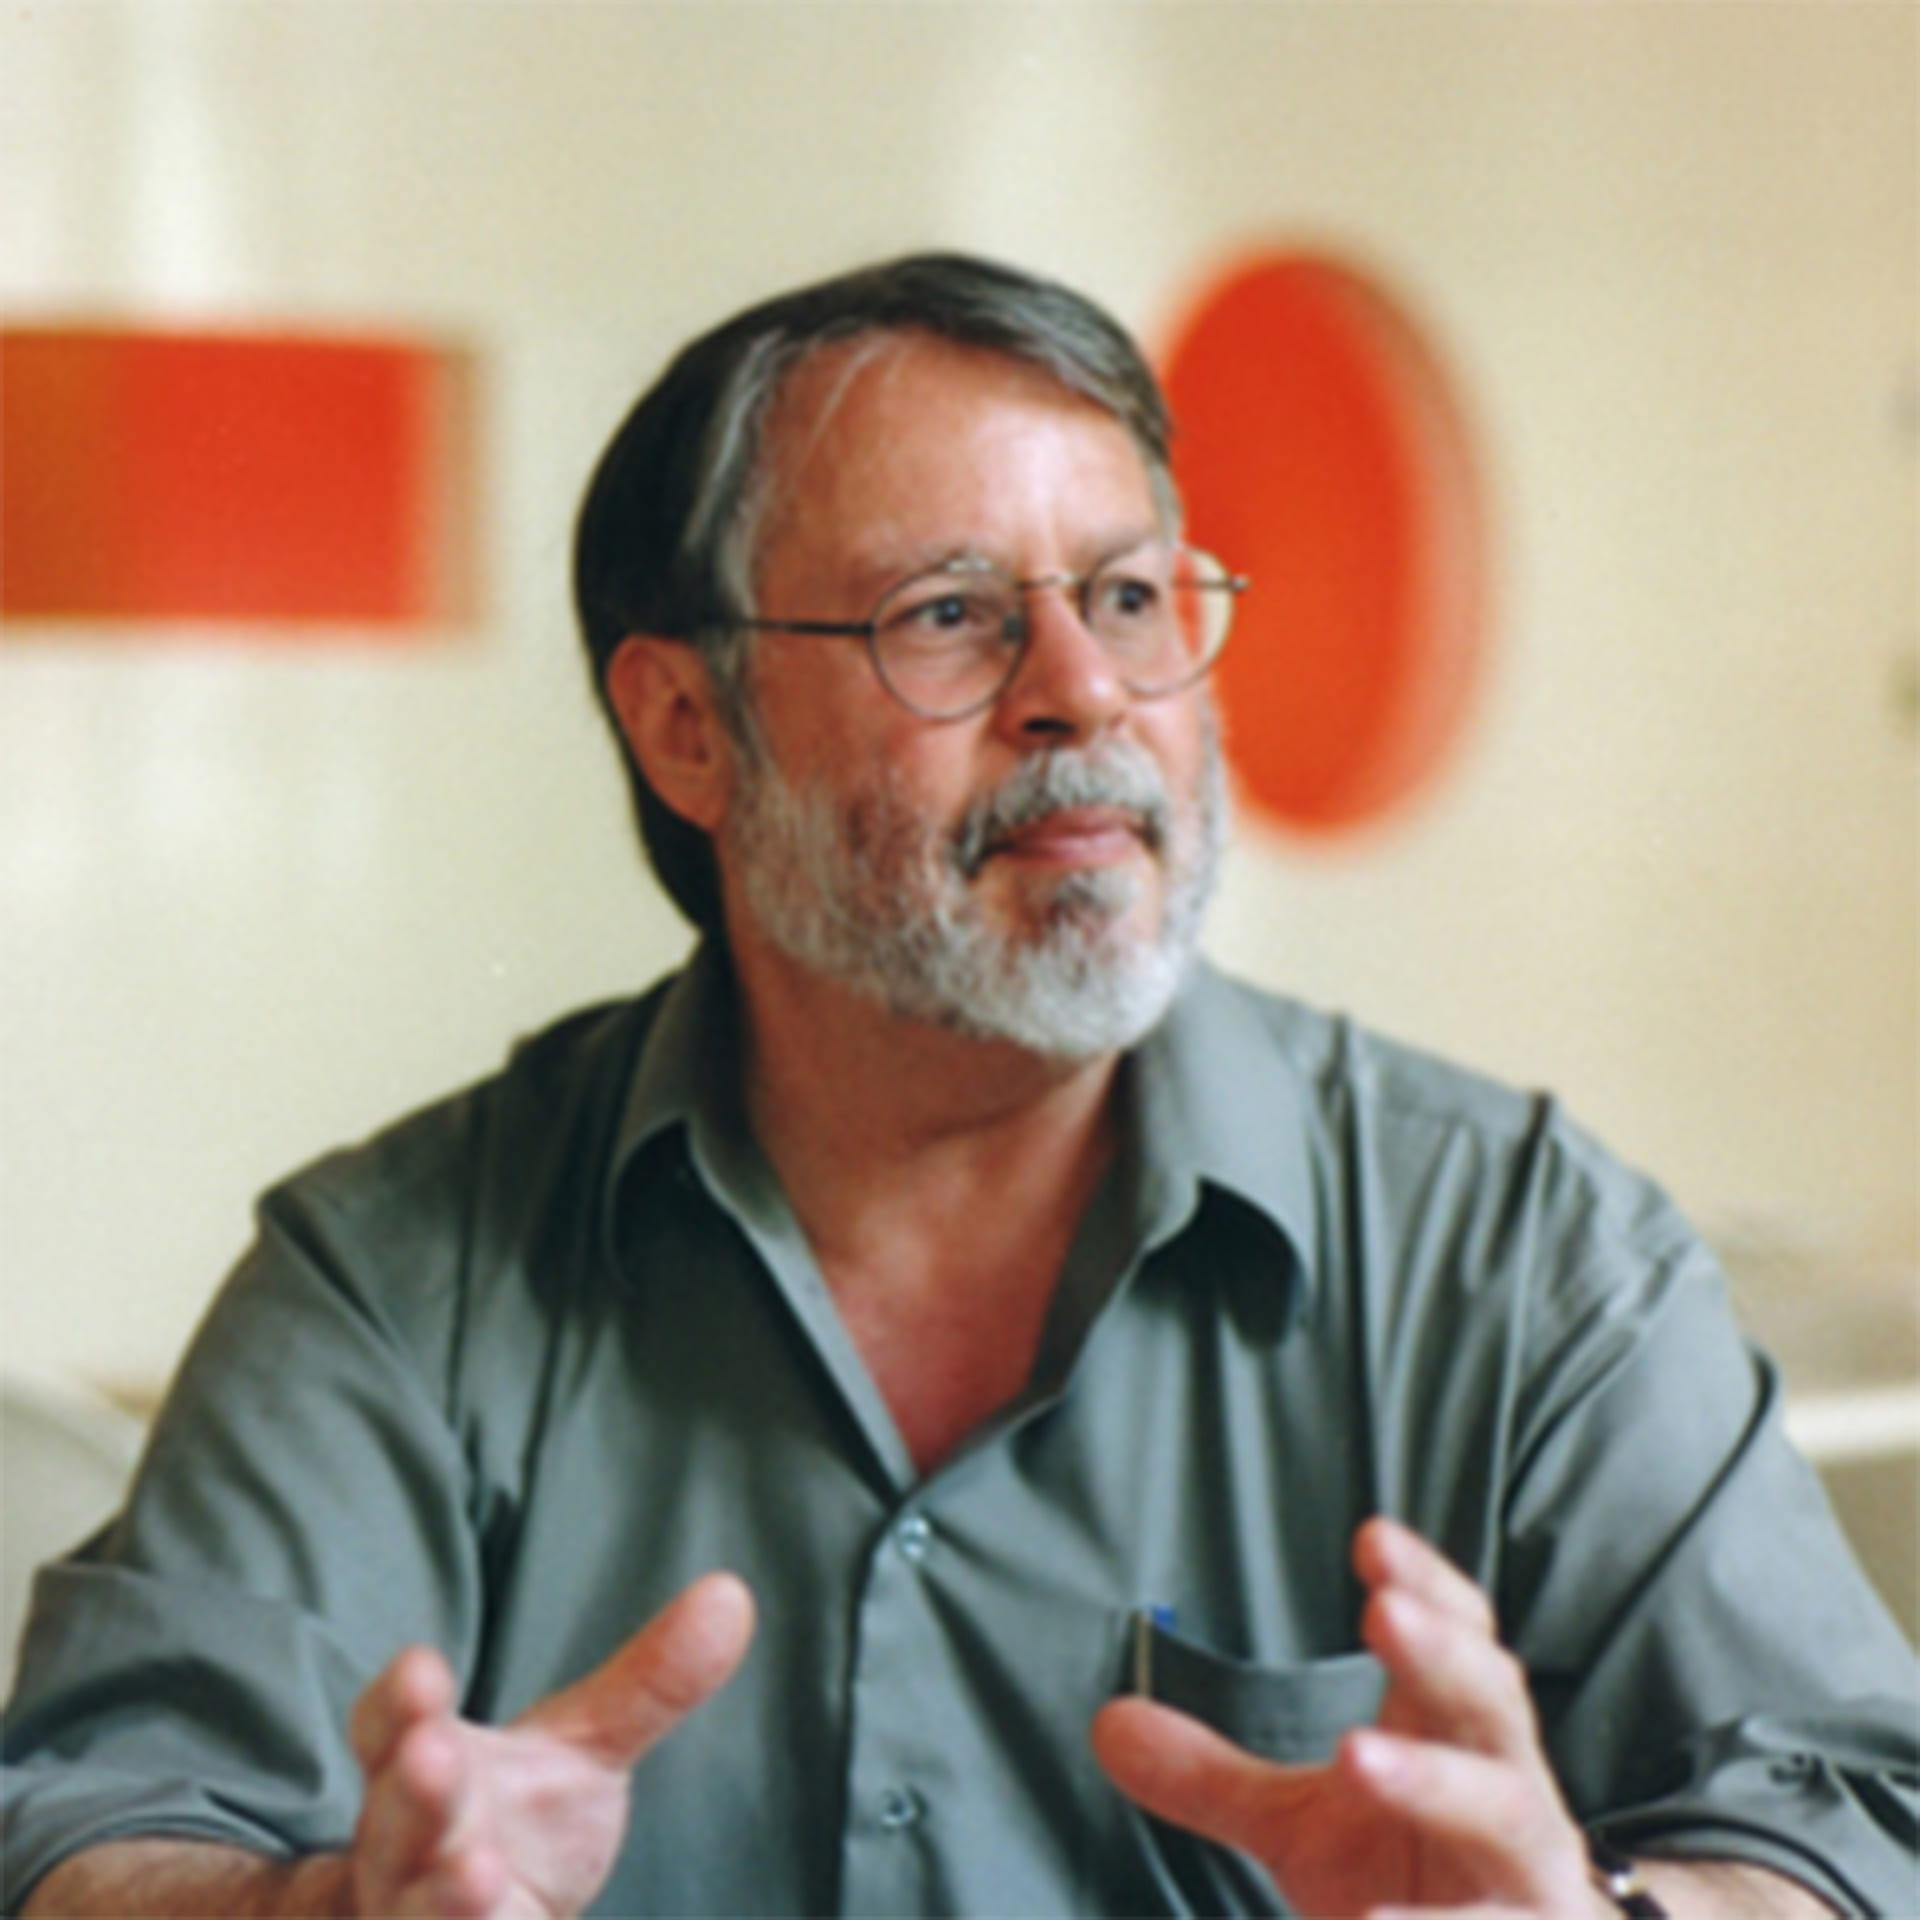
\includegraphics[width=.9\textwidth]{figures/liberman.jpg}
  \caption{Mark Liberman}
  \label{fig:ch.otlabphon.liberman}
\end{wrapfigure}
There had long been a feeling that \isi{syllable} structure ought to be
recognized explicitly in \isi{phonological representations}; yet the only
apparent way of doing that (by the use of intercalated \isi{syllable}
\isi{boundaries} in the segmental string) seemed cumbersome and
unenlightening. The recognition of hierarchical (or metrical)
structure in the domain of \isi{stress}, however, suggested that syllables
could be regarded analogously, as units defining a hierarchical
organization of segments into a larger structure. The first major step
in this direction was taken by \citet{kahn:thesis}, and was actually
formulated in terms of an \isi{autosegmental theory}
(section~\ref{sec:autosegmental}), but subsequent development has been
more in line with {\Liberman} and {\Prince}'s metrical theory.

With this enrichment of phonological organization, the hierarchical
representation of the relations among syllables could be annotated as
a relation of strong to weak, and this organization could be
interpreted as relative \isi{stress}, instead of treating \isi{stress} as a
feature like others.

At one shot, this theoretical move (which came to be known as the
theory of \emph{Metrical Phonology}) resolved all of the problematic aspects
of \isi{stress} in the purely featural account. It also, however, opened the
door to other innovations based on attributing more structure to
\isi{phonological representations} than that of a single uniform matrix of
features.  Metrical phonology was an immediate success.  Analyses of a
variety of languages in these terms were produced, and something of a
consensus about the range of possible \isi{stress} systems in the languages
of the world emerged in Bruce \posscitet{hayes:thesis} dissertation a
few years later.

\begin{wrapfigure}{r}{.35\textwidth}
  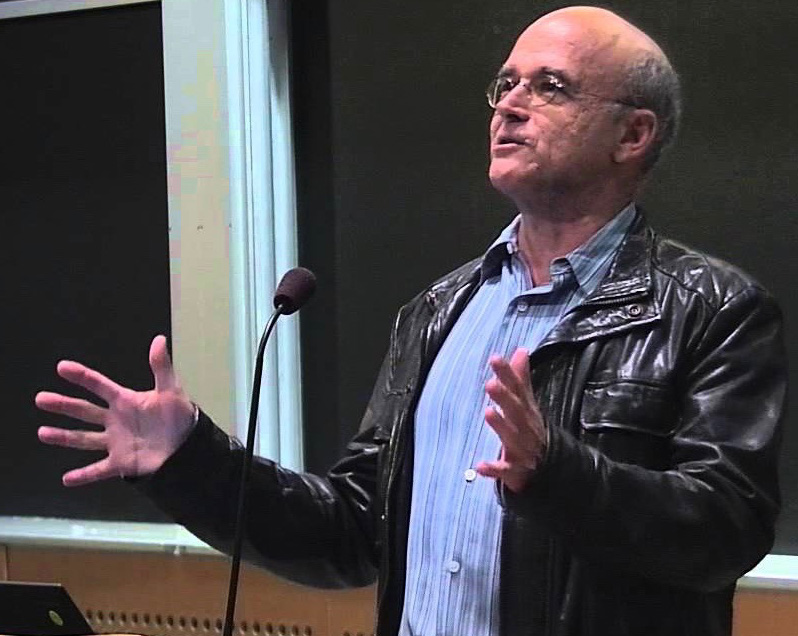
\includegraphics[width=.9\textwidth]{figures/Alanprince.jpg}
  \caption{Alan Prince}
  \label{fig:ch.otlabphon.prince}
\end{wrapfigure}
A variant of metrical \isi{representations} already foreshadowed in its
presentation by \citet{liberman:prince:stress} was the treatment of
rhythmic phenomena in terms of a grid, rather than hierarchical
constituent structure. This was developed and extended to other
properties by \citet{prince:grids}; after an initial burst of
enthusiasm, however, work in this framework has generally been quite
limited.

In {contrast}, the recognition of syllables and higher metrical
constituents such as feet and prosodic words as structurally
significant units was taken up widely and quickly became part of the
basic vocabulary of phonological description. The absence of
syllables, etc., from \isi{phonological representations} in \textsl{\isi{SPE}} was
not, as some have suggested, a matter of oversight or ignorance on
{\Chomsky} and {\Halle}'s part. Rather, it constituted a principled
decision: insofar as all generalizations apparently requiring
reference to units other than segments could be encoded in terms of
segments alone without significant loss of generality, the more
limited theory constituted a stronger empirical claim about the nature
of language. It seemed to {\Chomsky} and Halle that this was correct; and
at minimum it represents a coherent position.

The emerging work in Metrical Phonology, however, made it clear that
phonological analysis could not proceed without recognizing a variety
of structural units hierarchically organized above the level of the
segment.  The theory of these prosodic categories (foot, prosodic
word, phonological phrase, etc.) was organized in work such as
\citet{nespor:vogel:prosodic:phon}, and the relation of hierarchical
prosodic structure to similar structures in syntax was explored by
\citet{selkirk84:book}.

The success of Metrical theory in resolving problems in the analysis
of \isi{stress} led to a flurry of efforts to apply the new formalism to a
range of familiar problems. Vowel harmony, for instance, was described
(by \citealt{halle.vergnaud81:harmony}) as involving in some languages
the assignment of a harmonic feature to the head of a metrical tree,
and its subsequent propagation through the structure by
convention. Other, similar developments are suggested in papers in the
two-volume collection of papers by
\citet{struct_phon_rep_I,struct_phon_rep_II}. The wisdom of extending
metrical formalisms into all of the traditional segmental domains
where such formulations were proposed was questioned by
\citet{sra:ruletypes} and \citet{poser:distance}, and the exuberant
expansion of metrical accounts was somewhat short-lived. While it is
obvious that these formalisms do have considerable relevance beyond
the facts of \isi{stress}, subsequent work largely abandoned the attempt to
expand metrical analyses beyond essentially suprasegmental phenomena.

\subsection{Autosegmental Phonology and structure within the segment}
\label{sec:autosegmental}

The new perspective on \isi{stress} and other prosodic systems provided by
the richer notions of structure in Metrical and Prosodic Phonology
encouraged students to look for other areas in which comparable moves
would provide better accounts of problematic phenomena. Such a domain
was the analysis of tonal systems: like \isi{stress}, tonal features seemed
to be associated with phonological content in ways that were not
satisfactorily represented by features of individual segments.

Early attempts to incorporate tonal phenomena in generative
descriptions, such as the proposals of \citet{wang67:tone.features},
described tones as unitary features. In fact, Wang proposed that these
features should be attached to syllables rather than to segments, but
this aspect of his theory went essentially unnoticed in the
literature. There were no such things as syllables in \isi{representations};
besides, the same results could usually be obtained by associating the
tone features with the segment(s) that constituted the \isi{nucleus} of the
\isi{syllable}.

Wang\ia{Wang, William S-Y.}'s claim that tones---especially contour tones, such as the
rising, falling, and falling-rising tones of \ili{Mandarin Chinese}—could be
represented as units in a feature system was challenged in a
dissertation by \citet{woo69:thesis}.\footnote{The question of whether
  tonal contours should be seen as units or sequences of \isi{levels} has of
  course been raised by numerous scholars, including among others
  {\Trubetzkoy}, {\Sapir}, {\Pike}, {\Hjelmslev} and {\Martinet}. We confine our
  discussion here to the way this issue played out in the generative
  literature, without \isi{meaning} to imply that it was first discovered
  there.} She argued that contours should not be regarded as single
units but as sequences of (level tone) units. A falling tone is seen
not as a single element characterized by some feature such as
{[H-fall]} but as a sequence of a high tone followed by a low. On the
assumption that tone \isi{levels} are associated with units of vocalism, Woo\ia{Woo, Nancy}
argued that syllables bearing complex tonal contours always contain at
least enough vowel segments (or moras) to support the tones in a
one-to-one fashion.

Shortly thereafter, work on the tonal systems of African languages by
\citet{leben71:thesis} and others demonstrated that such contour tones
need to be recognized as also occurring on syllables containing only a
single, indivisible, short-vowel segment. Given the decomposition of
contours into sequences of \isi{levels}, it is necessary to admit the
possibility that some phonological features (such as the individual
subparts of a contour tone) take as their domain of specification a
scope less than a single segment (see also
\citealt{sra78:tone_features}). Segments, in other words, have to be
recognized as having significant internal temporal structure. On the
other hand, {\Leben} also showed that it is sometimes necessary to
recognize a single tonal specification which takes more than a single
segment as its domain, possibly spreading over several syllables of a
form.

To accommodate these and similar observations, John
\citet{goldsmith:thesis} proposed a view known as \emph{Autosegmental
Phonology}, on which rather than all being present in unitary columns
of the representation, individual features were linked to one another
by association lines. Within such a framework, a single specification of one feature
could be linked to one or more specification(s) of other features, thus allowing
for a tonal value to take a number of segments as its unitary domain.
Alternatively, multiple values of a single feature could be linked to a single
specification of some other, thus allowing for the description of
contour tones as sequences of \isi{levels} associated with a single
vowel. The traditional columnar view of \isi{representations} then
corresponds to the limiting case where all associations between
features are one-to-one.

\begin{wrapfigure}[15]{l}{.4\textwidth}
  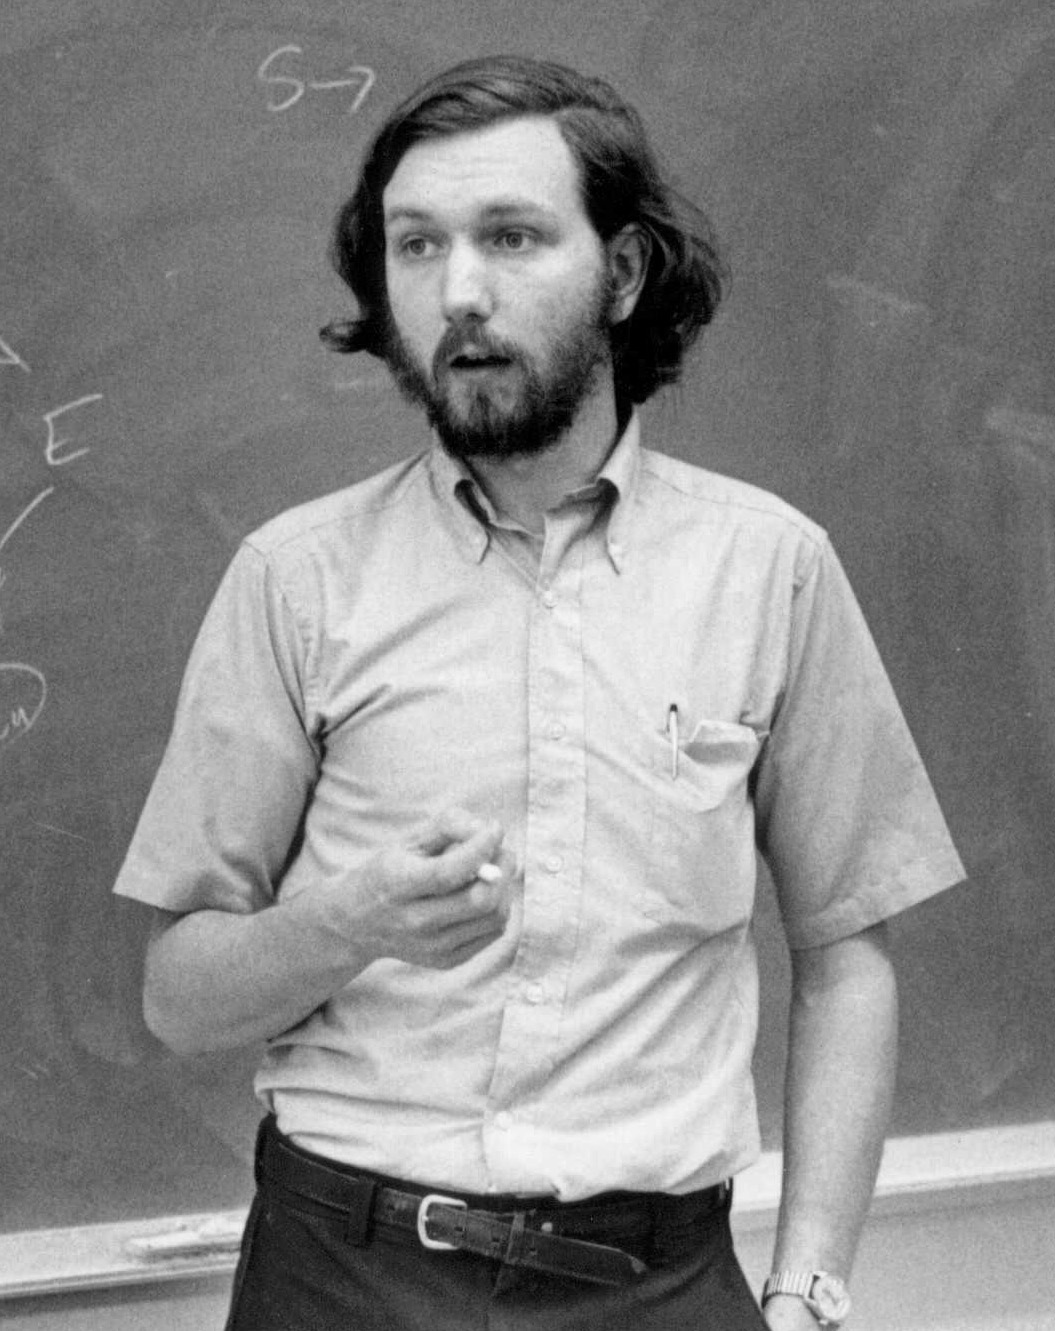
\includegraphics[width=.9\textwidth]{figures/goldsmith_1978.jpg}
  \caption{John Goldsmith (1978)}
  \label{fig:ch.otlabphon.goldsmith}
\end{wrapfigure}
While initially motivated by phenomena of tone, the apparatus of
Autosegmental Phonology was soon pressed into service for a variety of
segmental processes. It is clear that once we accept the claim that
the number of tonal specifications on a given form is not necessarily
equal to the number of vowels, the possibility arises of extending the
same descriptive formalism to other areas of structure. Nasality, for
example, provides a ready analog to the behavior of tones (see
\citealt{sra76:nasals}, as well as {\Goldsmith}'s work). Others,
particularly \citet[and elsewhere]{clements76:vowel.harmony}, have
argued that \isi{vowel harmony} provides another example of a single
phonological feature specification whose scope is not just a single
segment, but as much as an entire word.

As, a result of these developments, phonologists had come by the late
1970s to regard \isi{representations} less as a sequence of segmental `beads
on a string' than as analogous to an orchestral score in which the
synchronization of each instrument with the other instruments is as
much a part of the score as the actual notes each is to play. In
phonological terms, the `instruments' are the various separable
components of the speech apparatus: the laryngeal control of pitch,
the velum, the tongue body, the lips, etc.

A wide variety of phenomena take on a rather different appearance when
seen in this way. For instance, rules of \isi{assimilation} can often be
regarded as involving not a change in the features of some individual
segment but a re-association of the features of one segment (the one
assimilated to) so that they come to include the other (assimilating)
segment in their scope. In fact, there are few rules in the
phonologies of the moderately well studied languages whose form
remains unaffected when considered in terms of the manipulation of
autosegmental structure and associations rather than as changes in the
values of features.

\largerpage
As work of this sort developed, the question was raised of which
features tend to associate together, and which independently. This in
turn led to the proposal that the features themselves are organized
into a sort of tree structure, such that for instance a node {[Place]}
dominates a number of features specifying \isi{place of articulation}, and
can associate as a unit (in e.g. nasal \isi{assimilation} from a following
obstruent). The proposal of such organization produced the program of
\emph{\isi{Feature Geometry}} as introduced by \citet{clements85:geometry},
\citet{sagey90:thesis-garland} and others. The research agenda set by
this view was to uncover a single uniform organization of features
into higher-level categories valid across languages; despite
considerable effort, however
(e.g. \citealt{mccarthy:feature-geometry}), such an organization did
not emerge, and work in this program declined rapidly.

Throughout the period discussed here in
section~\ref{sec:representations}, we can note an evolution of
theoretical concern within the general framework of this book. The
\textsl{\isi{SPE}} program laid out a structurally simple, homogeneous
theory of phonological and \isi{phonetic representations}, and taking that
as a given, concentrated its attention on capturing putative
generalizations made by speakers, formulated as rules. Most of the
theoretical apparatus of \textsl{\isi{SPE}}, therefore, is developed to
articulate the character of \isi{phonological rules}. To the extent
representational issues arise, these concern the extent to which
\isi{phonological representations} can be allowed to deviate from surface
phonetics, but the answers to such questions are assumed to fall out
from the operation of the system of rules.

\largerpage
The reactions to this program articulated in different ways by
\citet{kiparsky:3dimensions} and \citet{hooper:ngp}, discussed above
in sections~\ref{sec:abstractness} and~\ref{sec:ngp}, shifted
attention to a concern with the \isi{abstractness} of phonological
\isi{representations}, but remained within an overall framework in which the
grammar as a system of rules was the primary object of study. The
development of Metrical and Autosegmental phonology, however, and
other research programs such as that of \isi{Feature Geometry}, resulted in
a wholesale shift of attention to representational matters. As
\citet[84]{mccarthy:feature-geometry} put it, ``During the last 10
years or so, phonological theory has made great progress {[\ldots]} by
adhering to two fundamental methodological premises. The first is that
primary emphasis should be placed on studying phonological
\isi{representations} rather than rules. Simply put, if the \isi{representations}
are right, then the rules will follow. The entire theory or research
program known as nonlinear phonology is based almost entirely on this
idea.'' This development from a concern with rules to a focus on
\isi{representations} would be taken still further in the novel views that
began to appear by the end of the 1980s.

Each of the theoretical innovations just surveyed resulted in an
initial burst of enthusiasm and proliferation of research results. As
the work became more standardized, however, phonologists sought out
new topics, sometimes leaving problems of the previous round of
innovation unresolved --- just as the move to richer theories of
representation had left behind unresolved problems of the \textsl{\isi{SPE}}
theory, such as the relation of \isi{notational conventions} to special
principles of application, the nature and generality of rule interactions,
and others. In some cases innovations left their traces in the general
view, as with the acceptance of much of the apparatus of Metrical,
Prosodic and Autosegmental theory in forming a broadly accepted view
of phonological structure. By the early 1990s, however, the field ---
which had become accustomed to a rapid turnover of ideas and research
topics --- was in need of a new infusion of both, and had begun to
develop a sense of stagnation. What happened then represented a more
extreme change than anything since the appearance of \textsl{\isi{SPE}}.

\section{The rise of Optimality Theory}
\label{sec:rise-ot}
\largerpage
During the 1980s, a great deal of artificial intelligence research
within the computer science community was focused on the development
of the architecture of neural networks
\citep{rumelhart.mcclelland86:pdp}, ``Connectionist'' systems that
were claimed to be able to learn, on the basis of exemplars as
training data, complex associations between inputs and outputs without
explicit instruction in the nature of the relation involved. One
application of this work was in the analysis of natural language, and
an influential paper in that framework
\citep{rumelhart.mcclelland86:past} claimed to document such a system
that acquired a significant segment of the morphology of \ili{English} (past
tense forms of verbs) without direct instruction apart from a training
set. The assumptions and adequacy of this model were strongly
criticized by \citet{pinker.prince88:connectionism}, and linguists and
cognitive scientists generally were not impressed with the promise
this approach might hold for their fields.

Among those in the computer science community engaged in the
exploration of neural network models, \name{Paul}{Smolensky} had especially
broad interests in cognition more generally, and in particular in the
nature of the \isi{representations} that could be attributed to these models
and ways in which symbolic processes could be modeled. When he
as a prominent Connectionist, and \name{Alan}{Prince} as a prominent critic of
that approach, met and began to work together, there was actually a
substantial amount of common ground for them to explore.

\begin{wrapfigure}[10]{r}{.4\textwidth}
  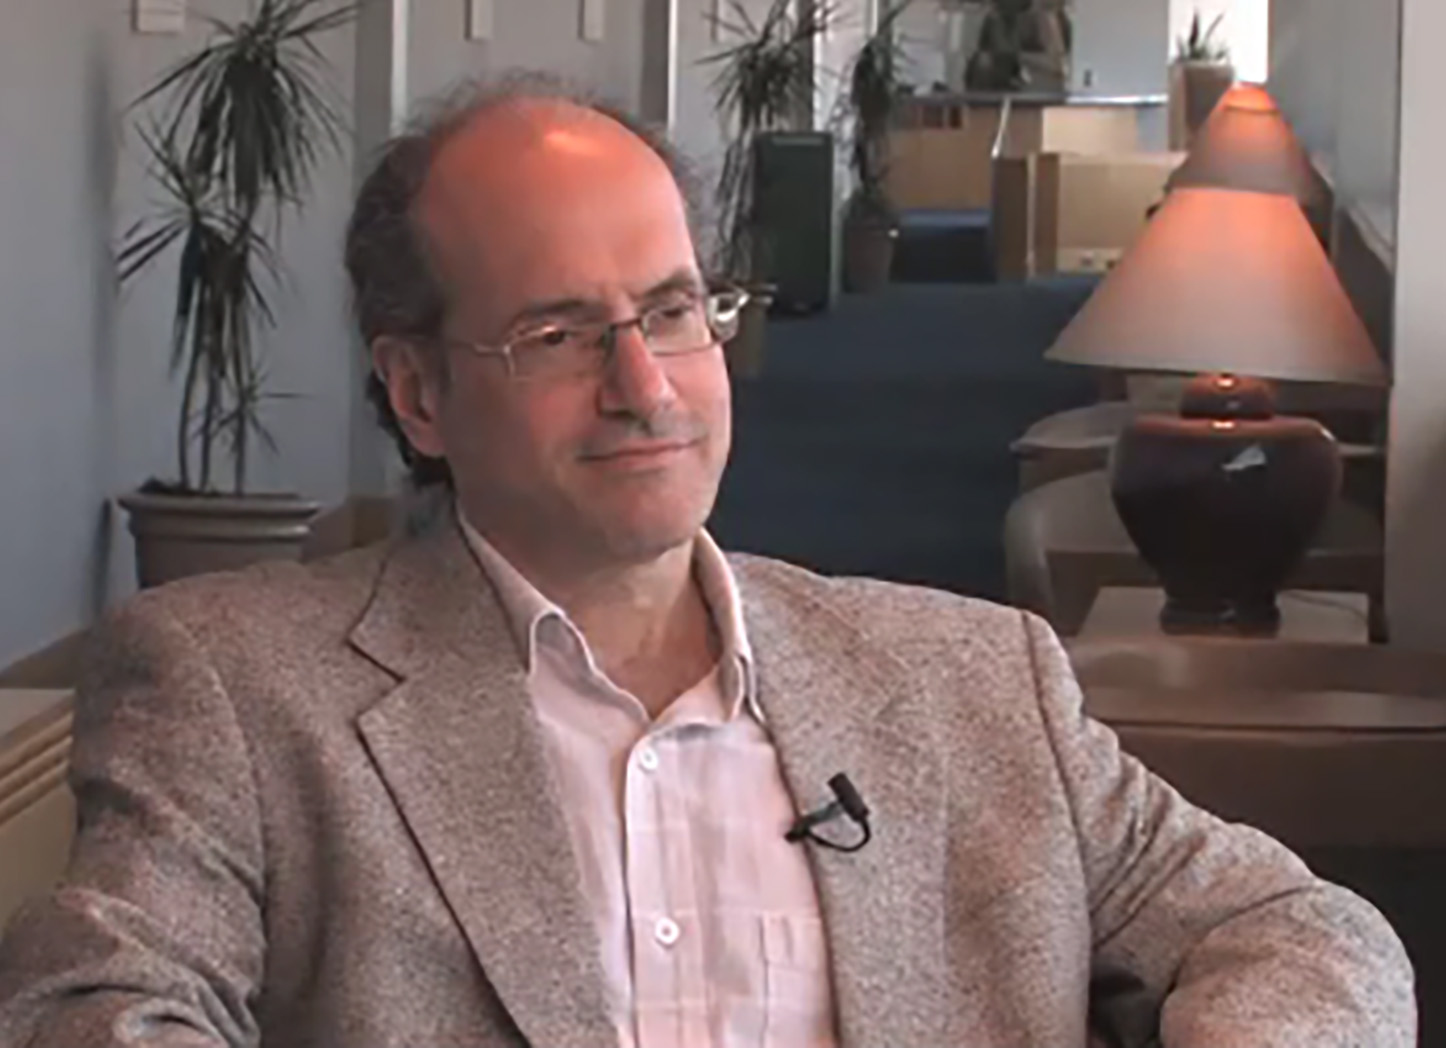
\includegraphics[width=.9\textwidth]{figures/smolensky.jpg}
  \caption{Paul Smolensky}
  \label{fig:ch.otlabphon.smolensky}
\end{wrapfigure}
After several years of collaboration, with occasional presentations to
other phonologists (e.g. in a workshop at the 1991 Linguistic
Institute at UC Santa Cruz), \citeauthor{prince:smolensky:optimality}
(\citeyear{prince:smolensky:optimality}; later published as
\citealt{prince:smolensky04:ot}) appeared as a photocopied manuscript
that was widely disseminated to large numbers of phonologists. This
set out a radically new approach to the description of phonological
systems, dispensing entirely with language-particular rules
functioning in a serial derivation.\footnote{For more detailed
  accounts than can be provided here of the rise of \isi{Optimality Theory}
  and of the theoretical proposals that preceded and anticipated it,
  see
  \protect\citealt{burzio_rise_1995,griffiths19:expansion-ot,vanOostendorp21:optimality}.}

The new framework was based centrally on generalizations about surface
phonetic forms, represented as \isi{constraints} taken from a universal
set. These were of two sorts: \emph{faithfulness} \isi{constraints}, which
require that the output phonetic form resemble the phonological input
in various ways, and \emph{markedness} \isi{constraints}, requiring the
output form to conform to various universal conditions of phonetic
\isi{naturalness}. These are typically in conflict with one another, and
thus must be ranked with respect to their importance: a grammar then
consists precisely of a ranking of the members of the universal set of
\isi{constraints}. A given constraint is allowed to be violated in the
surface form just to the extent this is required by other
higher-ranking \isi{constraints}. A derivation consists in taking a
phonological input form, allowing a component of the system
(``\textsc{Gen}'') to generate a potentially unlimited range of
possible corresponding outputs, and then evaluating in parallel each
of these against the ranked constraint set (``\textsc{Eval}''). The
candidate form whose constraint violations are least serious (the
``optimal'' candidate) is selected as the output.

It is not necessary for our purposes here to go into more of the
details of how such an \emph{Optimality Theoretic} (``OT'') grammar
works, and indeed subsequent developments have resulted in substantive
changes from the original mechanisms proposed by
\citet{prince:smolensky:optimality}. Some of these changes and their
motivations are sketched by \citet{vanOostendorp21:optimality}. What
is most important for present purposes is the fact that OT provided a
radically different account of phonological organization from that of
the \textsl{\isi{SPE}} model, even supplemented with all of the
representational innovations discussed above. The absence of language
particular rules, or any sort of serial derivational structure (at
least in the original formulation), combined with the focus on
surface-oriented \isi{constraints}, made this quite unlike anything that had
gone before, though it can in some sense be seen as the culmination of
phonology's shift in attention from theories of rules to theories of
\isi{representations}, sketched above in section~\ref{sec:representations}.

It is true that the potential importance of \isi{regularities} over surface
phonetic forms had been brought into discussion previously.
\citet{kisseberth:conspiracies} had noted in the early days of work
within the \textsl{\isi{SPE}} model that such \isi{regularities} sometimes did not
find any expression in such a grammar. Multiple rules might for
instance ``conspire'' to have the effect that \isi{stress} in a given
language never falls on a weak \isi{syllable} (sometimes moving the \isi{stress},
sometimes lengthening a vowel, sometimes deleting a \isi{syllable}, etc.),
but nowhere in the grammar is that stated in a unitary way, as for
instance by a constraint preventing stressed weak syllables. While
such ``conspiracies'' often seem to constitute quite real aspects of a
language's structure, the theory provided no effective way to
incorporate that observation into the description, and so it had to go
unstated. OT, in {contrast}, provided a clear status for such
generalizations.

It is also important to observe, as both
\citet{prince:smolensky:optimality} and
\citet{donegan.stampe09:hypotheses} do, the resemblance between OT's
positing a universal inventory of \isi{constraints} --- especially
\isi{markedness} \isi{constraints} --- and the system of natural processes in
\posscitet{donegan.stampe79:study.of.np} \isi{Natural Phonology}. In both
cases it is presumed that the intrinsic nature of the system
implementing speech has an important role to play in language, and
that the effects of this have to be ranked with respect to one another
and to the need to maintain distinct signals for distinct content (a
primary role of the faithfulness \isi{constraints}).

The universal nature of \isi{constraints} assumed in OT is not a
self-evident property of the theory. In particular, as analyses of
individual languages have proliferated within this framework, it has
become increasingly clear that the \isi{constraints} that need to be posited
for individual languages can in fact be quite specific. It is not
obvious that the assumption of a universal set of \isi{constraints} is other
than a place-holder for a system by which the \isi{constraints} active in a
given language could be learned --- a result that would {change} the
cognitive commitments of the theory in important ways and require more
attention to the characterization of possible \isi{constraints} than has
characterized the existing OT literature.

OT was also not the first phonological descriptive framework to focus
on \isi{constraints} as a formal method.
\citet{paradis.lacharite93:introduction} survey three such theories as
they existed at the time OT first appeared on the scene, including
Paradis's own (\citeyear{paradis87:constraints.and.repairs}) theory of
Constraints and Repair Strategies. Other frameworks relying heavily on
\isi{constraints} as opposed to derivational rules included those of
\citet{vennemann88:preference.laws} and
\citet{burzio94:english.stress}, but none of the others caught the
attention of the field in the way OT did.

A number of factors other than its intrinsic character conspired in
OT's success, as argued by \citet{griffiths19:expansion-ot}.  Along
the lines of other theoretical developments described earlier in the
present chapter, OT came along at a time when the field was eager for
something new. It was aggressively promoted by its originators, making
use of communicative channels (the Internet) that facilitated rapid
dispersion in ways unavailable to much previous theoretical
innovation.  Within a remarkably short time, most new work in
phonology was being produced in this framework.

Initially, on the basis of the illustrative analyses provided by
\citet{prince:smolensky:optimality}, OT appeared to be primarily
useful for the description of prosodic properties, including \isi{syllable}
structure and related effects. Soon, however, research had pushed the
techniques of the framework into essentially all areas of phonological
structure, and its victory was to all intents and purposes
complete. Some important linguists (including, notably, both {\Chomsky}
and {\Halle}) were unconvinced, and argued against OT, but others came on
board, and most importantly, students rushed to adopt the new approach
in formulating dissertation topics. By the end of the 1990s,
rule-based serial derivations were only to be seen in the work of a
few outliers, a state of affairs that continued well into the new
millennium.

\section{An alternative view: The Laboratory Phonology movement}
\label{sec:labphon}

Although differing in many essentials from preceding phonological
theories, OT can be seen as essentially developing a basic view of the
architecture of grammar similar in important ways to that of various
forms of ``Generative Phonology.'' Strongly contrasting with this
conception is that of the \emph{\isi{Laboratory Phonology}} movement, an
approach originating in the 1980s in work of a number of phoneticians.\footnote{This section has benefited from comments and
  suggestions by Bob {\Ladd}. The background and conceptual bases for the
  \isi{Laboratory Phonology} movement are discussed by
  \citet{dobrovolsky94:labphon.rvw} and
  \citet{pierrehumbert.etal00:labphon}. The first decades of research
  are summed up in papers presented at the 10th \is{Laboratory Phonology}LabPhon Conference,
  including retrospective essays by \citet{cohn10:labphon10.intro} and
  \citet{jbp.clopper10:what.is.labphon}. A comprehensive handbook
  covering a variety of topics within the general perspective has
  appeared as \citealt{cohn.etal11:labphon.hbk}.}

Unlike virtually all of the approaches considered up to this point in
the present work, \isi{Laboratory Phonology} should not be thought of as a
``theory'' of phonological structure. Rather, it is an overall set of
assumptions shared by a rather broad range of scholars in several
distinct fields: not only phoneticians and phonologist, but
psychologists, neuroscientists, speech scientists, and even some in
the medical professions. Within this point of view a variety of more
specific theories have been pursued, such as \emph{Articulatory Phonology}
\citep{browman-goldstein89:articulatory-phonology}, among
others. Common to these participants is a commitment to laboratory
investigation of the physical reality of speech. A series of (roughly
biennial) ``\is{Laboratory Phonology}LabPhon'' conferences---of which the 18th is to be held in
Seoul in 2022---provide gathering points for a diverse range of
perspectives.

Most theories of phonology conform to an overall pattern. Individual
meaningful elements of a language are assigned an abstract
representation that characterizes their distinctness from other such
elements. This is built from a set of discrete elements: unitary
phonemes, discrete values (perhaps binary) for features drawn from a
limited set, etc. These \emph{phonological} (or \emph{phonemic})
\isi{representations} are then related to a set of \emph{phonetic} \isi{representations}
by means of a system of rules, or evaluation over a set of
\isi{constraints}, or simple definitions of elements, etc. Phonetic
\isi{representations} are again drawn from a limited set, perhaps the
segment types in an IPA chart, perhaps discrete values for a set of
features which may or may not be entirely or partially the same as
those characterizing \isi{phonological representations}, but in any case
units provided by a theory of possible sounds in the languages of the
world. The phonetic representation, in turn, serves as the input to a
language-independent apparatus for speech, yielding physical events of
\isi{articulation}, \isi{acoustics} and perception.

On this picture, the language user's knowledge of a particular
language is characterized by the phonological and phonetic
\isi{representations} and the system characterizing their relation. In
particular, the measurable phenomena of speech are consequences of a
presumed universal, language-independent system whose overall
character (though not, of course, the details of specific grammars) is
general across the species.

Workers taking the \isi{Laboratory Phonology} point of view in search of an
understanding of the relationship between the cognitive and physical
aspects of human speech reject this picture, in whole or in
part. Centrally, they maintain that idiosyncratic specification
characteristic of a particular language or a particular talker's use
of the language affects speech implementation in potentially
continuous ways all the way down to the level of physical events which
can be measured and generalized over in statistical terms. Studying
speech in this way involves paying much greater attention to
\isi{variation}, within and between speakers and languages, than has been
characteristic of phonologists. This calls into question the usual
assumptions about a universally applicable set of discrete phonetic
categories:
\begin{quotation}
  One way of interpreting such results is as an indication that
  phonology proper covers less, and phonetic implementation covers
  more, than traditional approaches supposed. [\ldots] Experimental
  studies also show that there are no two languages in which the
  implementation of analogous phonemes is exactly the same. When
  examined in sufficient detail, even the most common and
  stereotypical phonetic processes are found to differ in their
  extent, in their
  timing, and in their segmental and prosodic conditioning\\
  \citep{pierrehumbert.etal00:labphon}
\end{quotation}
Arguably, then, the principal objection of Laboratory Phonologists to
more traditional views of phonology is grounded in their rejection of ``the
idea that there's a valid symbolic phonetic representation of any
utterance expressed in terms of a smallish finite set of universal
categories'' (Bob {\Ladd}, personal communication 7 May, 2021).

The goal of the initial organizers of the Laboratory Phonology
movement, including \name{Mary}{Beckman}, \name{Janet}{Pierrehumbert} and their
associates, was to remake phonology on the basis of a much richer
understanding of the observable reality of speech. What has happened
instead is that this has become a sort of sub-group among
phoneticians, such that phonologists who are mainly interested in the
forms of grammars continue to generate strings of phonetic symbols and
ignore what happens in their implementation, while those who focus
their research on measurable aspects of speech have little to say
about classical areas of phonology such as patterns of \isi{alternation}.
This is not absolute in either direction: \citet{ladd14:structure}
presents a position that falls generally within the Laboratory
Phonology view, but does not neglect the treatment of alternations,
while the papers in \citet{hayes.etal04:phonetic.phonology} address
classical phonological issues in terms of a close study of phonetic
detail.

Much work in this tradition proceeds with a general lack of engagement
with the phonological views that have been the object of current
phonologists' work, and \emph{vice versa}: there has in fact been very
little actual interaction between the two approaches beyond the
occasional appearance of phonologists at \is{Laboratory Phonology}LabPhon conferences in search
of phonetic data bearing on their categorial analyses.  Given the
tenuous connections between these two views, and the mutual
indifference that limits the content of the critical literature, a
more substantial consideration of the \isi{Laboratory Phonology} perspective
and related theories is beyond the scope of the present book.



\section{Conclusion}
\label{sec:conclusion}

In the developments reviewed above over more than a century, we can
find a considerable amount of progress in ideas that has, overall, led
to a richer and more substantial view of the sound systems of natural
languages. By no means all of what has been seen as progress, however,
can be attributed solely to the superiority of new approaches over old
ones in terms of their ideas. In some cases, we see that when the
problems arising within a theoretical perspective become sufficiently
complex, and the data necessary to resolve them too elusive, the
result is a search for a new research agenda that would allow students
to achieve results in quite another direction.  Science does,
undeniably, make progress, but at least some of this progress results
as much from a need for novelty as it does from a resolution of old
problems.

As I write, such a {change} may be taking place in phonology once again,
though no landmark work as significant as that of
\citet{saussure16:cours-original}, \citet{trubetzkoy39:grundzuge},
\citet{bloomfield:lg}, \citet{harris:methods}, \citet{spe} or
\citet{prince:smolensky04:ot} has appeared to incarnate it. While
still without doubt a widespread and influential theoretical position
among phonologists, \isi{Optimality Theory} too has begun to lose its
primacy. As was the case for earlier ascendant views, the theory has
reached a point where the outstanding matters of controversy are
somewhat obscure and hard to resolve. In addition, the important
phenomenon of \isi{opacity} --- generalizations that are importantly true,
but true in a way not susceptible of formulation in terms of surface
form --- has not received a satisfactory resolution, a problem already
anticipated by \citet{burzio_rise_1995}.  The intractability of this
issue has remained despite serious effort and attempts to incorporate
into OT such core aspects of previous theories  as serial derivation
\citep{mccarthy07:ot-cc}.

Partially in reaction to such accumulating problems, phonologists
(as well as some other linguists) have turned away from traditional
methodologies to seek solutions in computational analyses, statistical
inferences and the data-mining study of increasingly available large
corpora of language materials. It is far too early to say whether this
approach will succeed in replacing linguists' conceptions of
phonological structure with something quite different. While it may be
possible that long unresolved questions of phonological organization
will yield to these methods, the temptation to see in this turn yet
another search for low-hanging fruit is hard (for the present author)
to resist.


%%% Local Variables: 
%%% mode: latex
%%% TeX-master: "/Users/sra/Dropbox/Docs/Books/P20C_2/LSP/main.tex"
%%% End: 
 
